\section{Introducción}

\vspace{0.5cm}

\Large\scshape
\begin{center}
    Contexto global e investigativo para la realización del proyecto
\end{center}
\normalfont

\divider

El precipitado incremento de la población mundial en las últimas décadas, causado por el acelerado desarrollo tecnológico humano a partir de mediados del siglo XX, ha generado un exponencial aumento de demanda energética para poder satisfacer los constantemente crecientes requerimientos de la población. En respuesta a esta incrementada demanda del sistema energético mundial, los países comenzaron a crecer su capacidad instalada de plantas de generación en base a la quema de combustibles fósiles (petróleo, carbón, gas, etc.), sin tener en cuenta el catastrófico impacto que tienen sobre la biósfera terrestre sus grandes emisiones de gases de efecto invernadero, como dióxido de carbono y metano.\\

Hoy en día, más de medio siglo después, las consecuencias de este desmedido incremento del consumo global de combustibles fósiles se pueden observar claramente en la temperatura promedio del aire superficial de la Tierra, que ya es más de \SI{1}{\celsius} mayor a temperaturas medidas a principio del siglo previo (figura \ref{Temp_Tierra})$^{[OWID-CO2AndGreenhouseEmissions]}$, con algunos estimados conservadores de más de \SI{2.5}{\celsius} para finales de siglo$^{[ref 12 Wikipedia]}$. Los efectos perjudiciales de este incremento de temperatura se pueden ver en muchas partes, como la extinción de especies, el retroceso de los glaciares, el aumento de incidencia e intensidad de fenómenos climatológicos extremos (tormentas, sequías, olas de calor, etc.), entre muchos otros.

\begin{figure}[h]
    \centering
    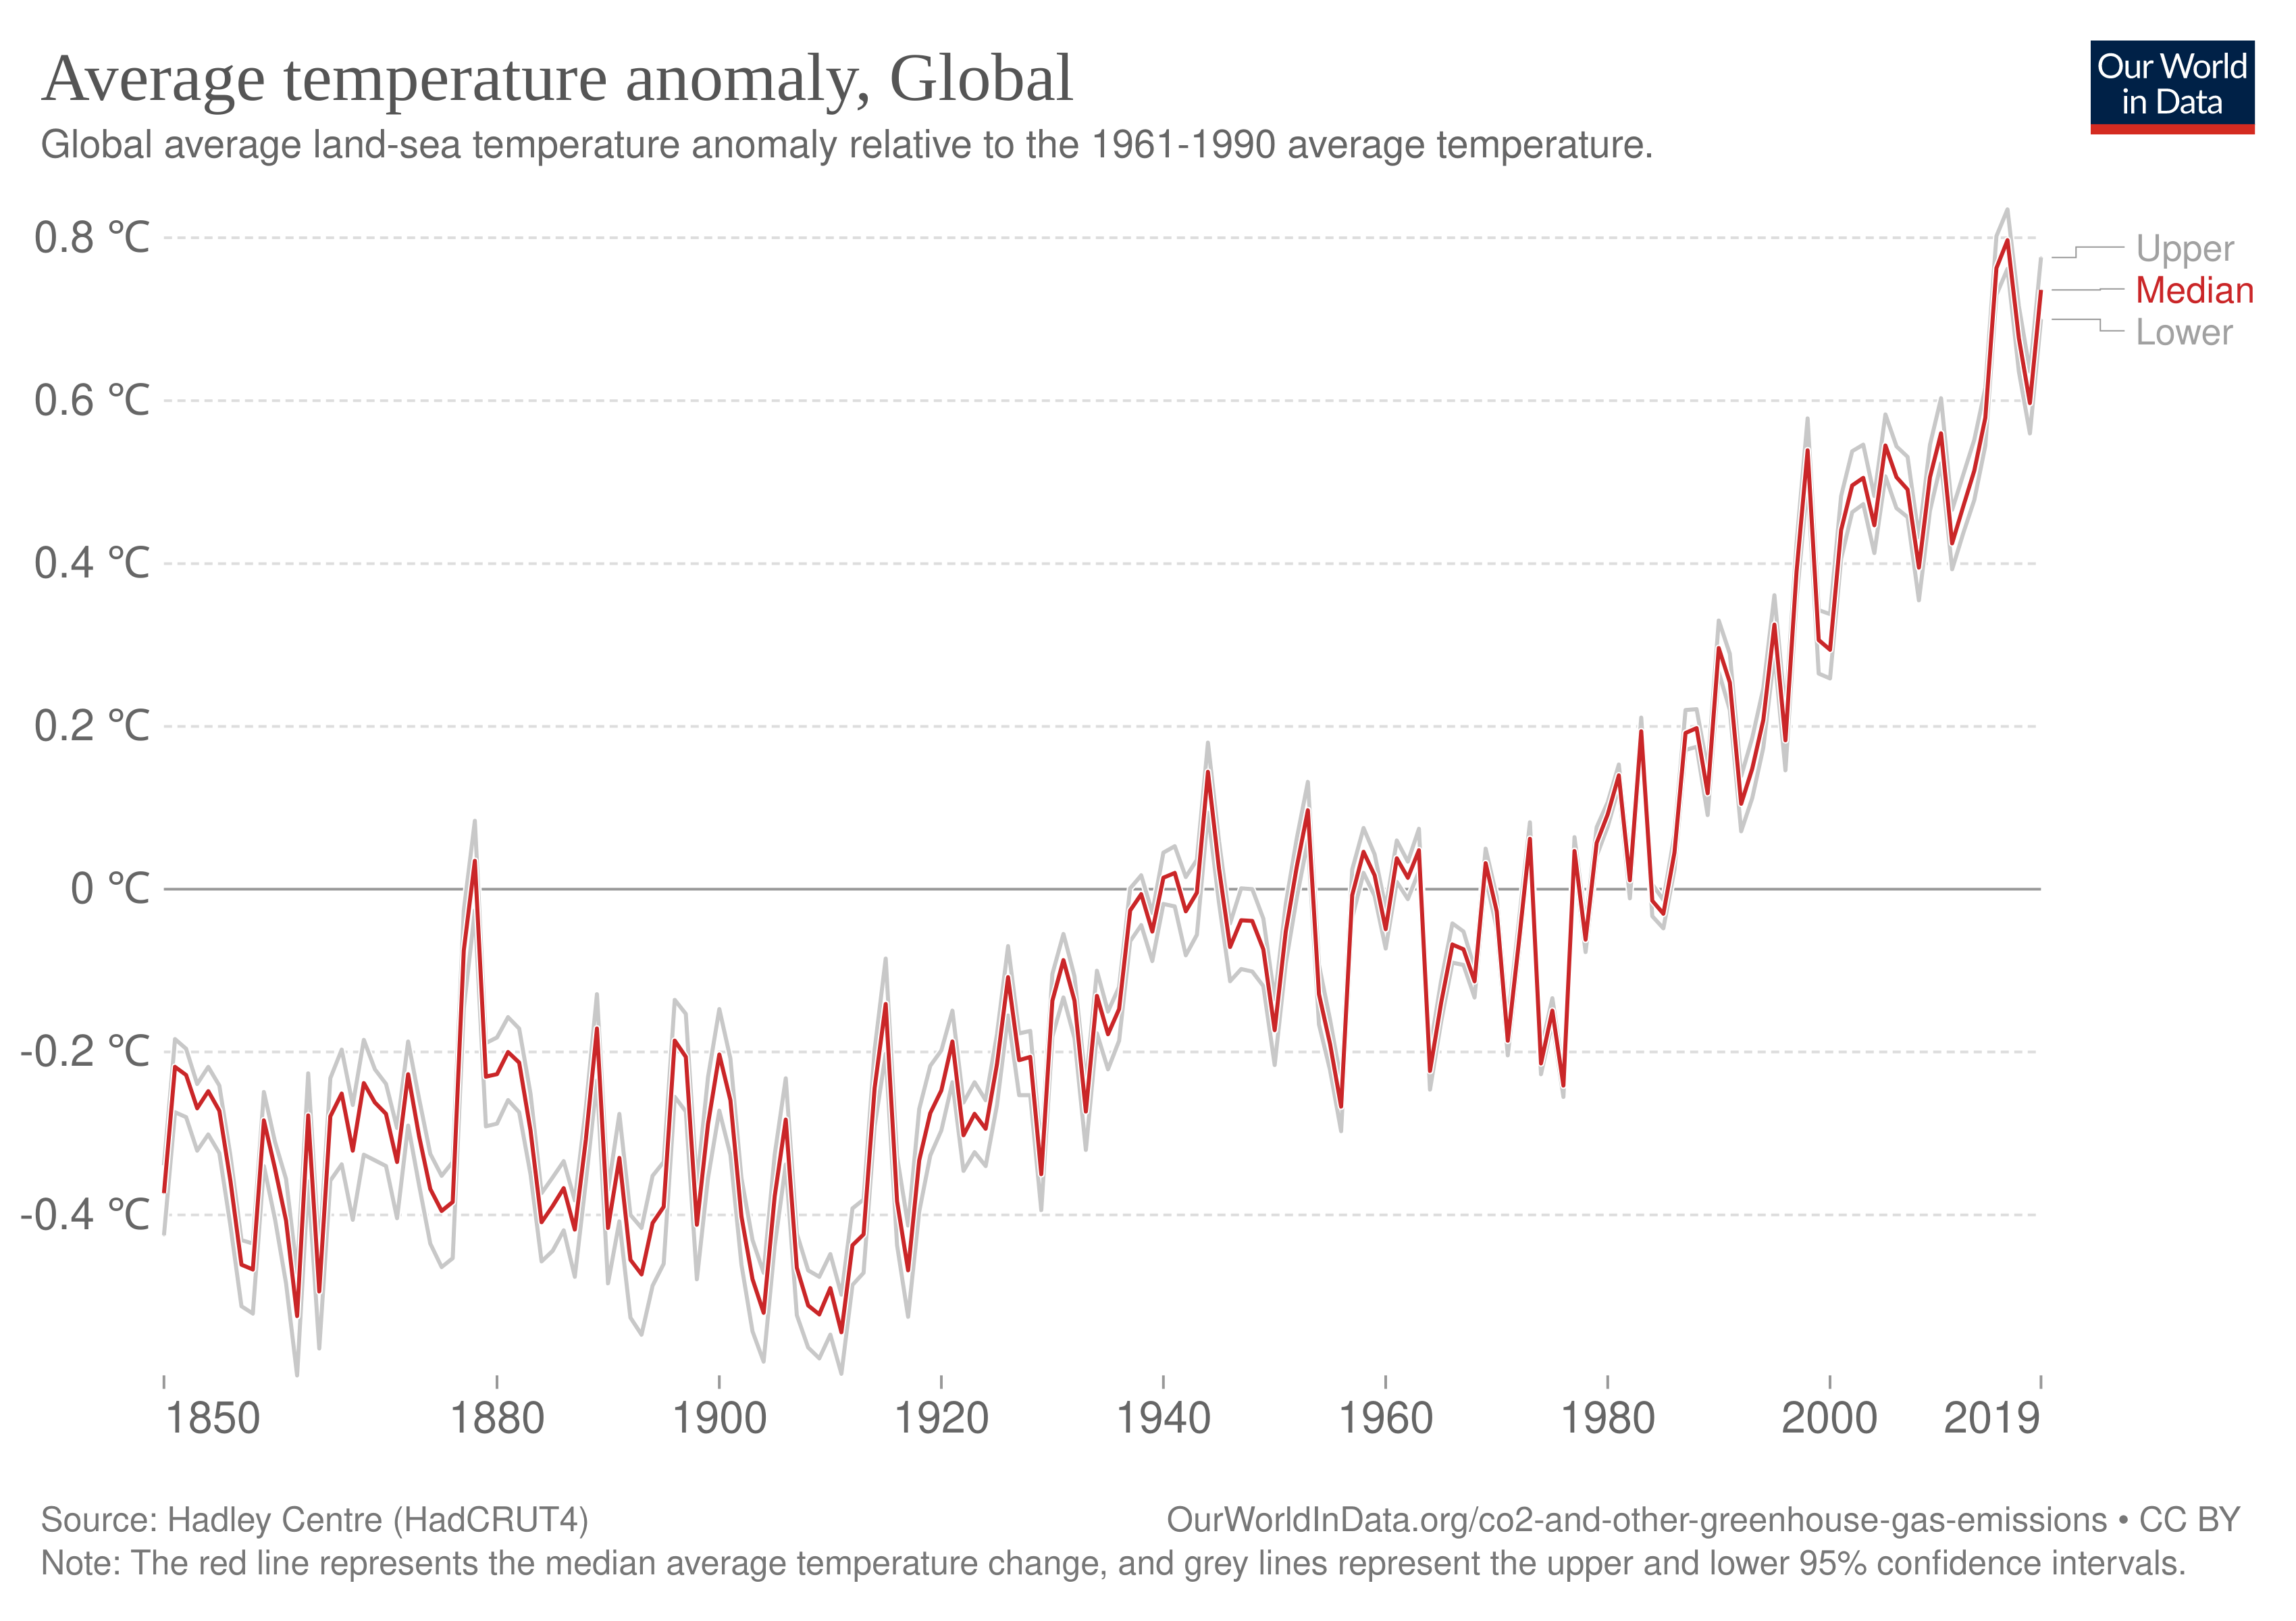
\includegraphics[scale=0.11]{Imagenes/Grafico Temperatura.png}
    \caption{Temperatura superficial promedio del planeta, relativo a la del período 1961-1990, desde 1850 hasta 2019.}
    \label{Temp_Tierra}
\end{figure}

Sin embargo, los combustibles fósiles y fuentes de energía no renovables siguen conformando una mayoría en el panorama de generación energética global: en el año 2019, alrededor del 85\% de la energía producida mundialmente provino de fuentes no renovables$^{[OWID-EnergyProduction]}$ (figura \ref{Emisiones_CO2}). Para frenar el avance del cambio climático, se debe acelerar el ritmo de adopción de energías alternativas como reemplazo de los combustibles fósiles, disminuyendo la emisión de CO$_2$ y metano en la atmósfera.

\begin{figure}[h]
    \centering
    \includegraphics[scale=0.11]{Imagenes/Grafico Fuentes de Energía.png}
    \caption{Consumo global de energía primaria según fuente, desde 1950 hasta 2019.}
    \label{Emisiones_CO2}
\end{figure}

Con esta motivación, el Instituto de Investigaciones en Electrónica, Control y Procesamiento de Señales (LEICI) de la Facultad de Ingeniería de la UNLP se embarcó en el proyecto ``Electrónica de Potencia y Sistemas de Control Avanzado Aplicados a Fuentes de Energía Alternativas'', dentro del cuál se enmarca el presente trabajo, que utiliza celdas de combustible en Sistemas Híbridos de Generación de Energía como fuente de energía alternativa.\\

\subsection{Sistemas Híbridos de Generación de Energía}

Un Sistema Híbrido de Generación de Energía (SHGE), en su descripción más general, es un sistema que combina distintas fuentes de energía, aprovechando las ventajas y suplementando las falencias de cada una de ellas. Generalmente, estos sistemas suelen combinar multiples fuentes de energías alternativas, como pueden ser, por ejemplo, generación solar mediante paneles y eólica mediante turbinas$^{[HybridEnergySystemModels]}$.\\

En nuestro caso, el sistema consiste en el módulo de generación principal basado en celdas de combustible, un módulo de generación alternativo como podría ser un sistema eólico o solar, un Sistema de Almacenamiento de Energía (SAE) basado en un banco de supercapacitores, y adicionalmente  un electrolizador para alimentar combustible a las celdas. Todos estos módulos son adaptados mediante sistemas de conversión eléctrica de potencia y conectados a un bus común de corriente continua (CC) con una tensión fija de \SI{75}{\volt} (figura \ref{SHGE}).$^{[2012Talpone][2019FIAnderson]}$.\\

En este sistema, el módulo de generación por celdas de combustible se encarga de entregar el nivel de potencia necesario para satisfacer la potencia demandada por la carga en el bus de CC. Mientras tanto, el módulo de generación alternativo tiene el rol de proveer potencia a la carga cuando el módulo de generación principal no es capaz de satisfacer por completo la demanda. El SAE aprovecha la capacidad de rápida de descarga de los supercapacitores junto con su alta capacitancia (almacena grandes cantidades de energía) para darle al SHGE velocidad de respuesta ante repentinos cambios de potencia demandada, a los que los módulos de generación no son capaces de responder a tiempo (luego, en momentos de menor demanda toma energía del sistema para cargar los supercapacitores). Finalmente, el electrolizador toma energía del sistema para generar el hidrógeno necesario para el funcionamiento de las celdas de combustible a partir de agua, mediante la reacción de electrólisis que se explicará en detalle más adelante$^{[2019FIAnderson]}$.\\

\begin{figure}[H]
    \centering
    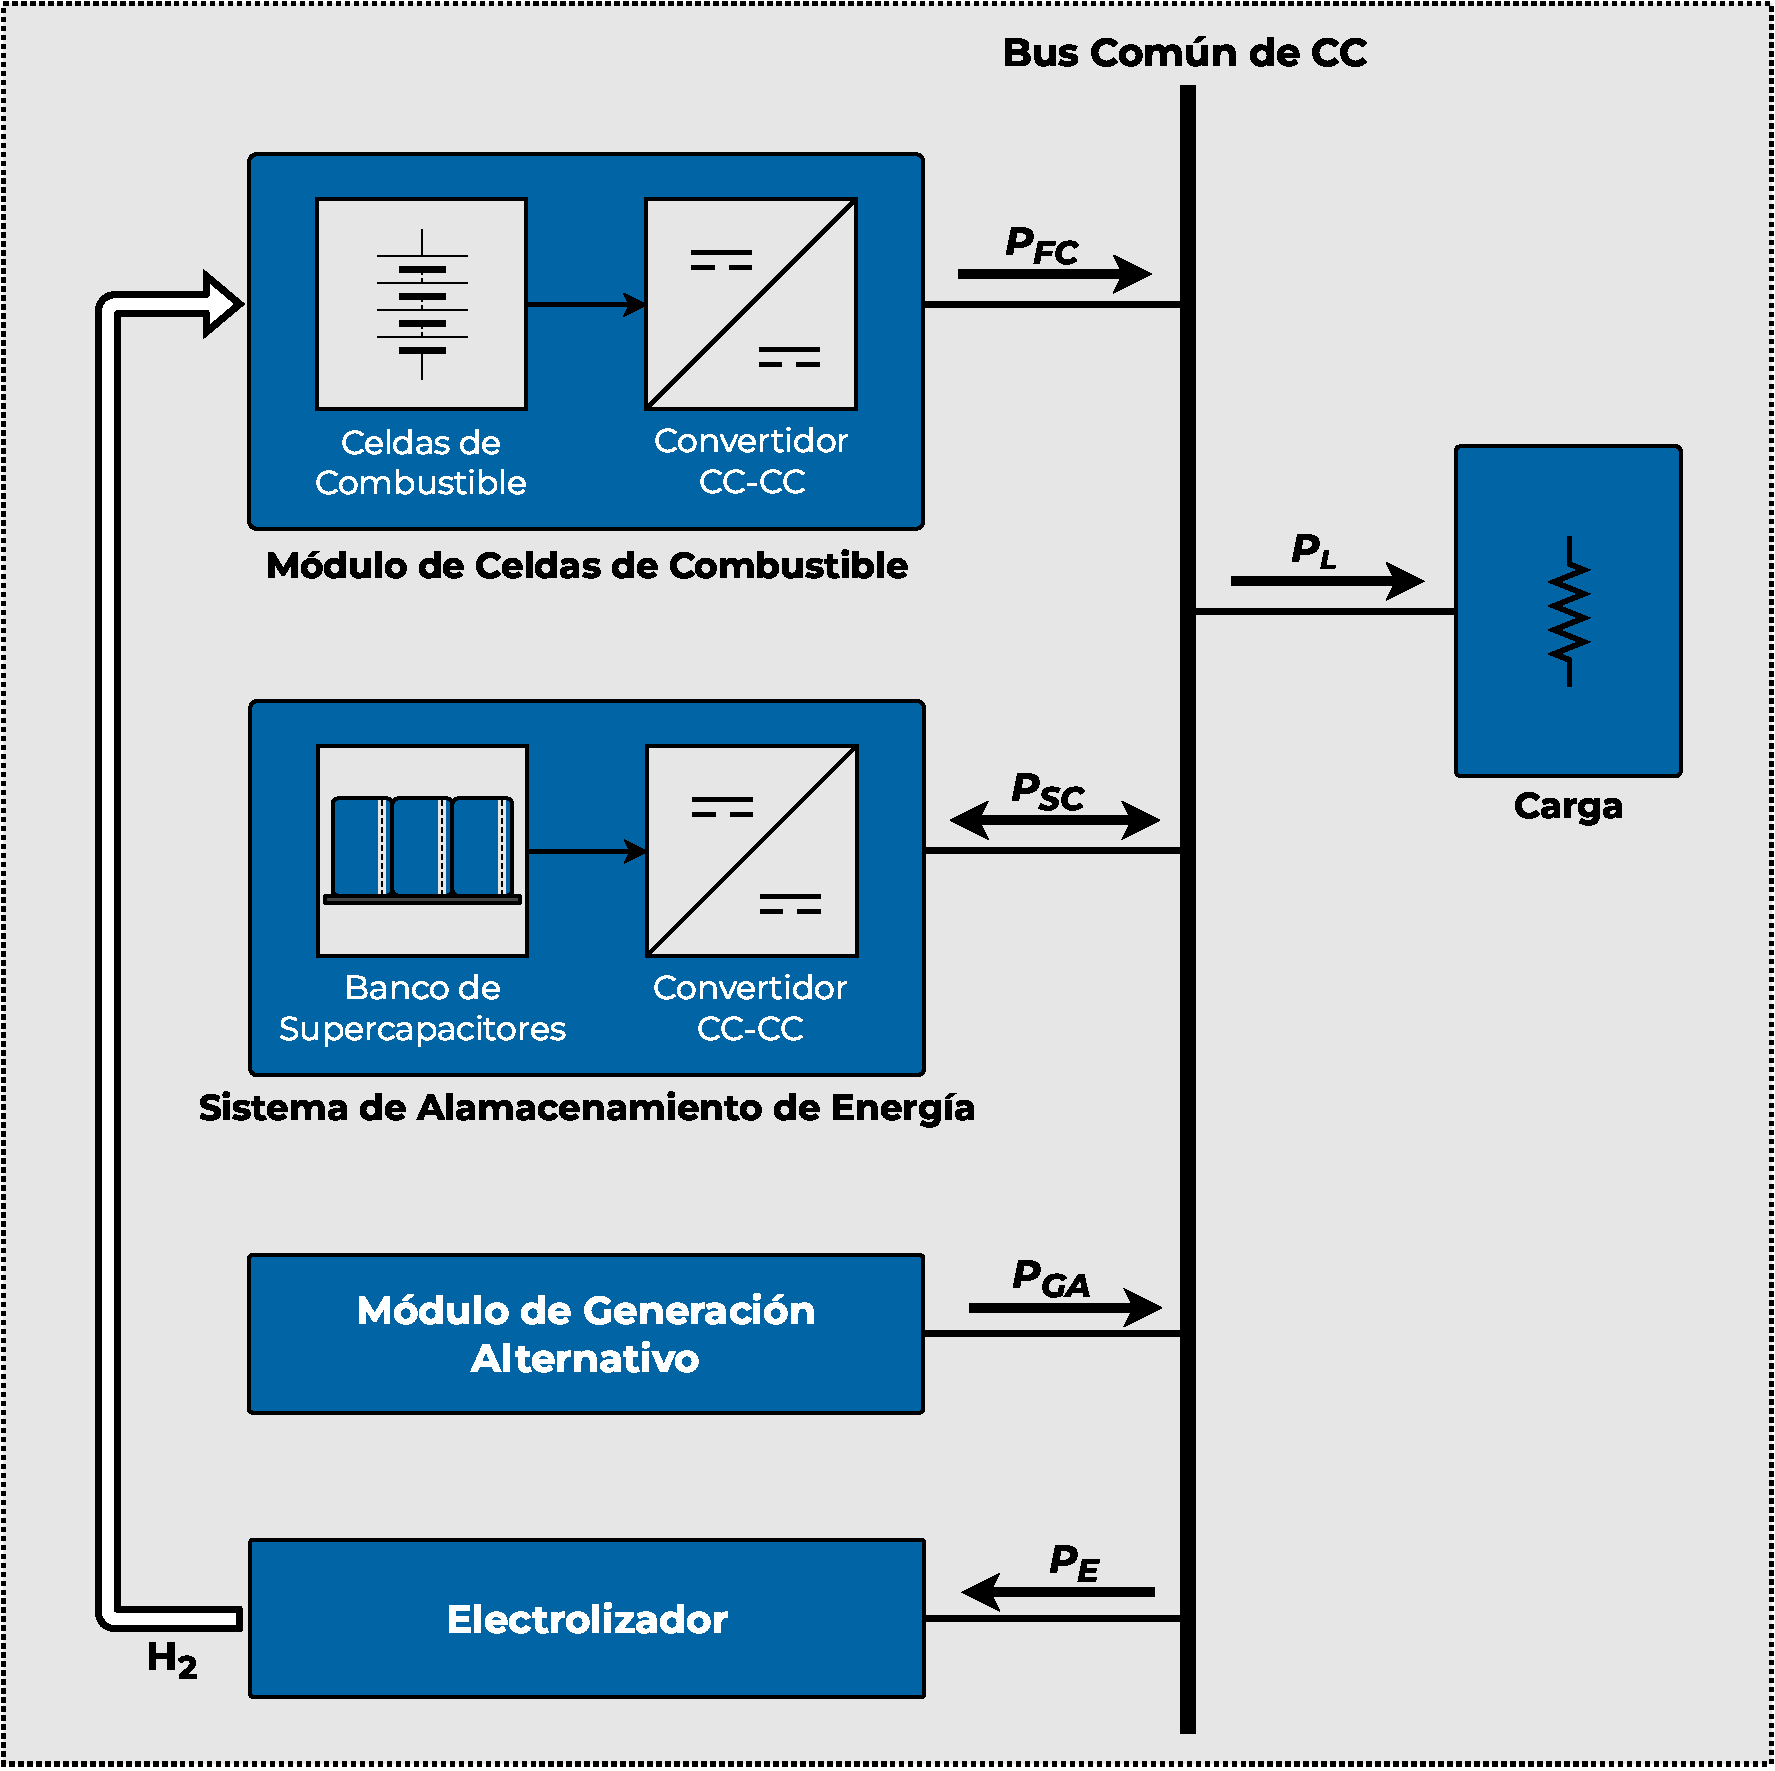
\includegraphics[scale=0.35]{Imagenes/SHGE.pdf}
    \caption{Sistema Híbrido de Generación de Energía (SHGE), con flujos de potencia indicados para cada módulo.}
    \label{SHGE}
\end{figure}

En particular, este trabajo se enfoca en el estudio, diseño, implementación y validación de una plataforma experimental para la evaluación del Módulo de Celdas de Combustible para sistemas híbridos de generación de energía.\\

Todo lo que refiere a esta plataforma se va a tratar en detalle a lo largo del desarrollo de los siguientes capítulos de este informe. Se comienza por un estudio en profundidad de la teoría de funcionamiento de sus componentes, pasando por una simulación de toda la plataforma para verificar su funcionamiento. Luego, se describe el proceso por el cuál se diseñó e implementó el sistema en una placa de circuito impreso (PCB, de \textit{Printed Circuit Board} en inglés); y se concluye el trabajo con la validación del correcto funcionamiento de la plataforma terminada.\\

